%!TEX root = ./Body.tex

\chapter{Verfahren} % (fold)
\label{cha:Verfahren}

Wollt ihr hier alle Verfahren haben, oder ein Datei für jeder?\\

blablabla


\section{K-Nearest Neighbor} % (fold)
\label{sec:KNN}
blablabla\\

blablabla
% section Verfahren1 (end)

\section{Random Forests} % (fold)
\label{sec:Forests}
blablabla\\

blablabla
% section Verfahren2 (end)

\section{Neuronale Netze Martin ODER KOMMT NIX?!} % (fold)
\label{sec:NN1}
blablabla\\

blablabla
% section Verfahren3 (end)

\section{Neuronale Netze} % (fold)
\label{sec:NN}
Künstliche Neuronale Netze nehmen das menschliche Gehirn als Vorbild und versuchen so eine Abstraktion von Informationsverarbeitung zu schaffen. Ein neuronales Netz besteht aus mehreren Schichten von Neuronen, die beliebig miteinander verbunden sein können. Zusätzlich zur Netztopologie wird noch eine Aktivierungsfunktion festgelegt, welche das „Feuern“ eines Neurons beschreibt. Der Ablauf bei dem Training des Neuronalen Netzes ist folgendermaßen: zuerst wird eine Netztopologie, eine Anzahl von Neuronen und die Aktivierungsfunktion festgelegt. Die Eingabewerte werden an die Neuronen der ersten Schicht (Eingabeneuronen) angelegt und mittels gewichteter Verbindungen und der Aktivierungsfunktion durch das Netz transportiert. Am Ende liefert die letzte Neuronenschicht (Ausgabeneuronen) einen Wert, welcher mit dem Soll-Wert verglichen wird. Das endgültige Lernen des Neuronalen Netzes ist nun die Anpassung der gewichteten Verbindungen zwischen den Neuronen des Netzes. Allerdings spielt auch die Netztopologie und die Anzahl der Neuronen eine wichtige Rolle. Eine genauere Beschreibung kann z.B. in (James A. Anderson: A simple neural network generating an interactive memory. In: Mathematical Biosciences. 14, 1972, ISSN 0025-5564, S. 197–220. ) nachgeschlagen werden.
Als Implementierung wurde das Framework von Boby Anguelov (http://takinginitiative.net/2008/04/03/basic-neural-network-tutorial-theory/) auf die Aufgabenstellung und die verwendeten Daten angepasst. Dieses Framework bietet ein dreischichtiges FeedForward-Netz und erlaubt eine variable Anzahl an Neuronen pro Schicht. Um die optimale Anzahl an Neuronen zu finden, werden optional sowohl konstruktive als auch destruktive Verfahren angeboten. Wie in Kapitel \ref{cha:Features} erläutert, wurde ein bestimmtes Set an Eingabevektoren ausgewählt und auch die Ausgabeneuronen waren durch die Anzahl der Stellgrößen vorgegeben. Weiterhin kann die Aktivierungsfunktion, sowie die Lernparameter wie Lernrate und Momentumterm angepasst werden. 

Der erste Teil des Trainings befasste sich also damit, die optimale Anzahl an Neuronen für unsere Aufgabenstellung und die Eingangsdaten zu ermitteln. Als desktruktives Verfahren wurde der Optimal Brain Damage Algorithmus (http://yann.lecun.com/exdb/publis/pdf/lecun-90b.pdf ) verwendet, als konstruktives Verfahren die Cascade-Correlation (http://www.cs.iastate.edu/~honavar/fahlman.pdf ). \\

\begin{figure}[!h]
	\centering
	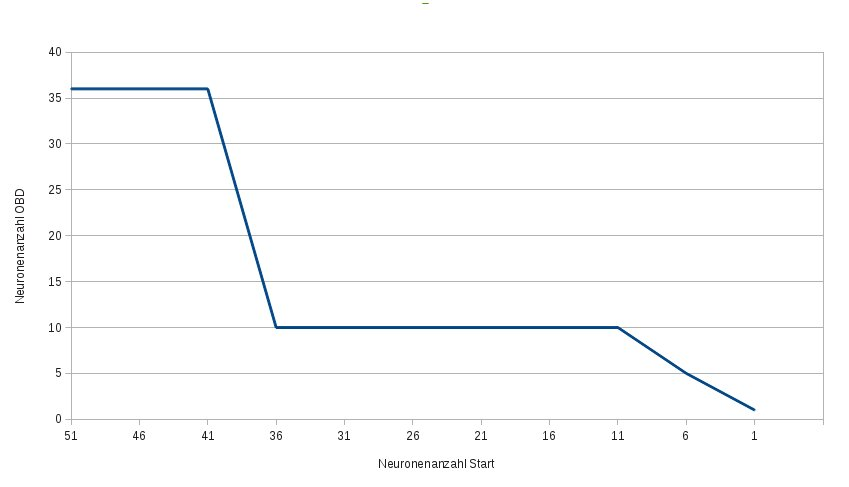
\includegraphics[scale=0.5]{images/nn/a1.jpg} 
	\caption{Ermittelte Neuronenzahl des OBD Algorithmus in Abhängigkeit der Startzahl an Neuronen}
	\label{nnchrisa1}
\end{figure}

Abbildung \ref{nnchrisa1} zeigt die von OBD ermittelte Anzahl an Neuronen abhängig von der Ausgangsneuronenanzahl. Es wird deutlich, dass ein Wert von 10 Neuronen vom Algorithmus als optimal aufgefasst wird; niedrige Werte verschlechtern das Ergebnis deutlich und auch höhere Werte sind bestenfalls gleichwertig. Allerdings benötigt das größere Netz deutlich mehr Zeit und auch eine größere Menge an Trainingsdaten.\\

\begin{figure}[!h]
	\centering
	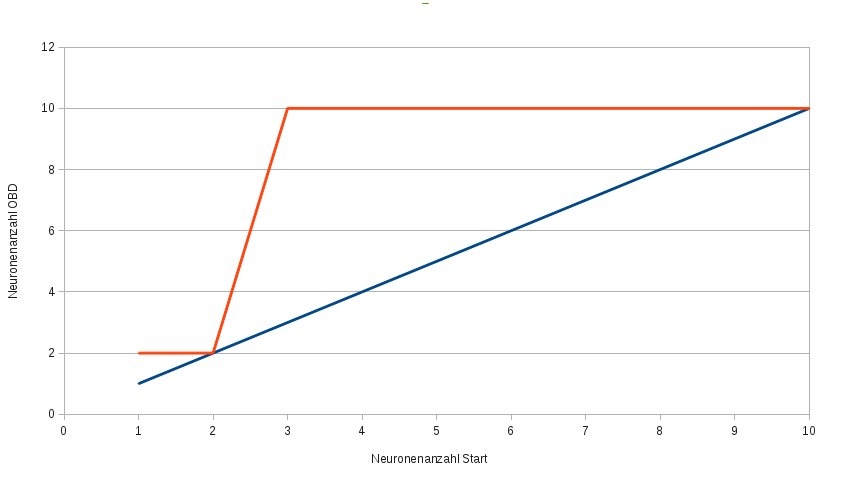
\includegraphics[scale=0.5]{images/nn/a2.jpg} 
	\caption{Ermittelte Neuronenzahl des OBD Algorithmus und des Cascade-Trainings in Abhängigkeit der Startzahl an Neuronen}
	\label{nnchrisa2}
\end{figure}

Abbildung \ref{nnchrisa2} zeigt jeweils die von OBD und dem Cascade Training ermittelte Neuronenzahl in Abhängigkeit vom Startwert für das Intervall zwischen 1 und 10 Neuronen. Das konstruktive Cascade Training lässt die optimale Neuronenzahl sehr deutlich gegen 10 konvergieren, welches vom OBD Algorithmus schon von oben eingegrenzt wurde. Für die weiteren Tests wurde also ein Netz mit 18 Neuronen verwendet, wobei 5 Neuronen als Eingabeneuronen, 10 Neuronen als Hidden-Neuronen, sowie 3 Neuronen als Ausgabeneuronen fungierten.\\

Mit dem festen Netzaufbau wurden nun die Lernrate und der Momentumterm untersucht. Das Training des Neuronalen Netzes wird mittels Gradientenabstieg vorgenommen. Bei diesem Verfahren wird versucht ein globales Minimum in der von den Fehlertermen aufgespannten Hyperebene zu finden. Folgende Probleme können hierbei auftreten:
Lokale Minima: Anstatt des globalen Minimums wird nur ein lokales Minimum gefunden und nicht mehr verlassen. Obwohl eventuell eine bessere Gewichtsverteilung existiert, wird diese nicht mehr gefunden.
Flaches Plateau: Wenn sich der Gradient über eine große Anzahl von Gewichtsanpassungen nicht mehr verändert, dann stagniert das Verfahren. Der Gradient wird so über weitere Schritte so klein, dass keine weitere Erforschung des Raumes mehr erfolgt.
Verlassen guter Minima: Falls ein ausgeprägtes Minimum mit relativ geringer Ausdehnung vorliegt, so kann es übersprungen werden. Also könnte auch so ein globales Minimum übersprungen werden.
Oszillation: Das Verfahren springt von einem Minimum in das nächste, wobei es zwischen beiden Minima hin und her springt. In diesem Fall verändern sich nicht die Beträge der Gradienten, sondern lediglich ihr Vorzeichen.
Eine hohe Lernrate ermöglicht ein schnelles Erforschen der kompletten Hyperebene des Fehlerterms. Flache Plateaus werden schnell durchlaufen und vom Startpunkt weit entfernte Minima werden schnell erreicht. Allerdings steigt auch die Gefahr gute (bzw. globale) Minima zu überspringen oder zwischen gefundenen Minima zu oszillieren. Bei einer Lernrate von 0.9 trat genau dies bei den Trainingsdaten auf. Das Training benötigte zwar nur eine kurze Zeit (eine Minute), allerdings zeigte sich dann eine komplette Oszillation.
Eine niedrige Lernrate kann komplexe Lerndaten, sowie eine große Datendichte besser bewältigen, ist weniger anfällig für Oszillation und für das Überspringen von Minima. Allerdings erhöht sich dadurch die Trainingszeit und Plateaus, sowie lokale Minima können nicht mehr überwunden werden. Dies zeigte eine Lernrate von 0.01 deutlich: das Training benötigte mehr als 12 Stunden und es wurde das „erstbeste“ Minimum nicht mehr verlassen.
Um die Nachteile einer niedrigen Lernrate auszugleichen, kann man ein Momentum einführen. Dieser Trägheitsterm berücksichtigt zusätzlich zur aktuellen Änderung des Gradienten auch die vorausgegangene Änderung. Hiermit wird ein schnelles überqueren von Plateaus ermöglicht.
Als endgültige Parameter wurden eine Lernrate von 0.1 und ein Momentum von 0.9 gewählt.\\

Die letzte Stellschraube des Lernverfahrens war die erlaubte Varianz im Vergleich der Soll- und Istwerte der Ausgabeneuronen. Da hier keine klassische Klassifikation, also ein binärer Vergleich, stattfand, sondern eine kontinuierliche Funktion gelernt werden sollte, muss dem Lernalgorithmen ein gewisser Spielraum gegeben werden. Weiterhin ist dieser Schritt damit motiviert, dass der Fahrsimulator nur Werte mit bestimmter Genauigkeit annahm, z.B. die Gaspedalstellung in Tausendstel-schritten. Eine hohe Varianz erleichtert natürlich das grobe Einlernen dieser Funktion, wobei eine niedrige Varianz die Funktion besser beschreiben sollte.\\

\begin{figure}[!h]
	\centering
	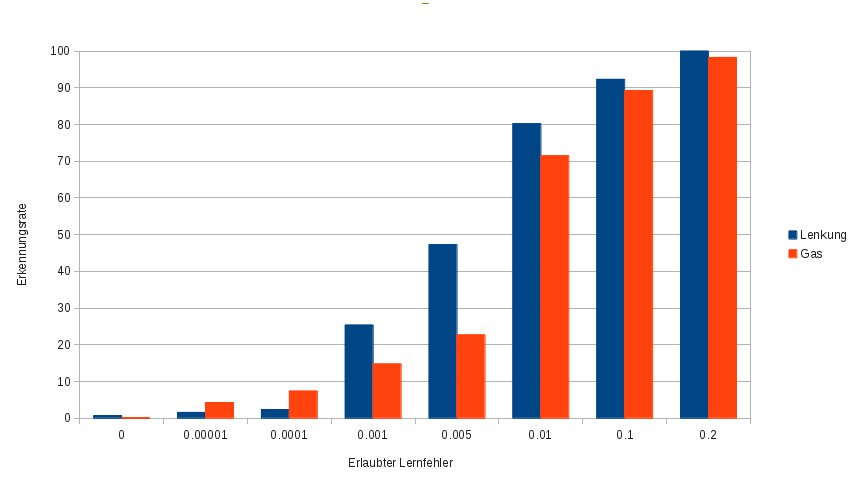
\includegraphics[scale=0.55]{images/nn/a3.jpg} 
	\caption{Erkennungsrate der Stellgrößen Gaspedalstellung und Lenkwinkel in Abhängigkeit der zugelassenen Fehlervarianz}
	\label{nnchrisa3}
\end{figure}

Abbildung \ref{nnchrisa3} zeigt die Erkennungsrate von Gaspedalstellung und Lenkwinkel in Abhängigkeit des erlaubten Lernfehlers. Eine allgemeine Aussage war hier nicht möglich, da in der Praxis die Gaspedalstellung mit wenig Fehlervarianz und somit niedriger Erkennungsrate, jedoch beim Lenkwinkel eine relativ hohe Fehlervarianz mit hoher Erkennungsrate besser funktionierte. 
% section Verfahren4 (end)

\section{Support Vector Regression} % (fold)
\label{sec:SVR}

\subsection{Lösungsstrategie}
\label{subsec:Lösungsstrategie}
Im Rahmen des hier vorgestellten Ansatzes wurde die \textit{Support-Vektor-Regression}, also die Regression mittels \textit{Support-Vektor-Maschinen} eingesetzt. Die erforderlichen theoretischen Grundlagen hierfür sind \cite{BenHur2008} entnommen. Eine ausgezeichnete praktische Einführung in die Thematik bietet \cite{HsuLibsvmTutorial2003}. Aus Gründen der Einfachheit sei die funktionale Umsetzung der SVR im folgenden Text durch die Abkürzung SVM beschrieben.
Das vorliegende Problem kann in eine Reihe von Teilproblemen zerlegt werden. So müssen zuerst der Ein- und Ausgaberaum bestimmt werden. Ersterer bezeichnet die Menge der Informationen, welche die jeweilige SVM zur Bestimmung ihrer Ausgangskenngröße nutzt. Letzteres ist vergleichbar zu den Stellgrößen, mit denen das Fahrzeug gesteuert wird und entscheidet über die Anzahl der verwendeten SVMs. Für jede SVM muss ein Kernel gewählt werden, der sich für die vorliegende Aufgabe eignet. Weiterhin müssen entsprechende Kernel-Parameter ermittelt werden.
In diesem Kapitel wird die Lösungsstrategie und das Vorgehen im Allgemeinen vorgestellt. Die beiden folgenden Kapitel beschäftigen sich mit der Parametersuche sowie der Strukturierung des Eingaberaums. Danach wird die praktische Umsetzung vorgestellt. Den Abschluss bildet die Diskussion der im Rahmen der Evaluation erzielten Ergebnisse.

\subsubsection{Kernel und Parameter}
\label{subsubsec:KernelUndParameter}
Die Wahl des passenden Kernels und der entsprechenden Parameter sind Gegenstand der aktuellen Forschung, daher hat sich dieser Teil als schwierig und sehr zeitaufwändig herausgestellt. Letztendlich wurde der \textit{RBF-Kernel} ausgewählt. Dieser erfreut sich großer Beliebtheit, da er zum einen nicht-lineare Entscheidungsgrenzen ermöglicht, zum anderen sehr wenige freie Parameter hat.
Für die Bestimmung der Kernel-Parameter wurden zwei Verfahren ermittelt, die im nächsten Kapitel ausführlich beschrieben werden. Die Bestimmung von Kernel und Parameter sind essentiell für das weitere Vorgehen, da sie die Evaluation einer gegebenen SVM erlauben. Dies ist vor allem für Experimente hinsichtlich der Struktur des Eingaberaums zwingend notwendig.

\subsubsection{Ein- und Ausgaberaum}
\label{subsubsec:EinundAusgaberaum}
Vor der Strukturierung von Ein- und Ausgaberaum muss zuerst entschieden werden, ob eine \textbf{Modellierung des Fahrzeugs} oder eine \textbf{Modellierung des Fahrers} gewünscht ist. Es wurde beschlossen, zuerst nur das Fahrzeug zu erlernen, da dies das einfachere Problem von beiden ist. Die Lösung des komplexeren Problems, nämlich das Erlernen des Fahrers war dann letztendlich aus Zeitgründen nicht mehr möglich.
Für das Erlernen des Fahrers ergaben sich hinsichtlich des Ausgaberaums zwei mögliche Varianten. Die wohl einfachste Lösung ist es, je eine SVM für die drei Ausgangsgrößen Gas, Bremse und Lenkrad zu trainieren. Dies hat den den klaren Vorteil, dass Gas und Bremse gleichzeitig angesteuert werden können. Dies ist z.B. für Ralley-Fahrer notwendig, die schnell aus einer Kurve beschleunigen möchten.
Da eine solche Möglichkeit laut Aufgabenstellung jedoch nicht explizit vorhanden sein muss wurden Gas und Bremse zusammengefasst. Die neue Ausgabestellgröße entspricht Gas minus Bremse (beide Stellgrößen wurden auf das selbe Intervall skaliert), wobei positive Werte eine positive Beschleunigung in Fahrtrichtung bedeuten und negative Werte das genaue Gegenteil.
Die Dekodierung auf die Stellgrößen Gas und Bremse erfolgt durch eine einfache, der SVM nachgeschaltete Logik. Dieses Vorgehen hat den Vorteil, dass nur für zwei SVMs Parametersuche  und Training durchgeführt werden müssen.
Zusätzlich zu den hier beschriebenen wurden weitere Ansätze angedacht. So war es beispielsweise vorgesehen,  ein Fahrzeugmodell (z.B. das Einspurmodell) zu nutzen, um darauf aufbauend mit SVMs den Fahrer zu erlernen. Eine Umsetzung war aus Zeitgründen leider nicht mehr möglich.

\subsubsection{Evaluation}
\label{subsubsec:Evaluation}
Die Evaluation der Ergebnisse wurde auf zwei unterschiedliche Arten durchgeführt. Im Rahmen der \textit{Offline-Evaluation} wurde der \textit{Mean Squared Errors (MSE)} mittels Kreuzvalidierung auf ein zufälliges Testset berechnet. Außerdem wurden für jede SVM die Ausgaben zusammen mit der Referenz geplottet und so eine Möglichkeit zur visuellen Inspektion gegeben. Dies hat sich als äußerst nützlich erwiesen, um Fehler aufzuspüren.
Bei der \textit{Online-Evaluation} werden die SVMs zur Fahrzeugsteuerung genutzt, Dies geschieht im Fahrsimulator. Die vom Fahrzeug gefahrene Trajektorie wird aufgezeichnet und mit der Referenz-Trajektorie verglichen. Hierzu lassen sich die durch das Framework zur Verfügung gestellten Funktionen nutzen.

\subsection{Parametersuche}
\label{subsec:Parametersuche}
Bedingt durch die Regression und den RBF-Kernel gibt es drei freie Parameter, die bestimmt werden müssen. Der Parameter \textbf{C} gibt die Kosten an, mit denen die Abweichung eines Punktes von der Hyperebene belegt wird. Die Kosten fließen jedoch nur dann ein, wenn die Entfernung mehr als \textbf{Epsilon} geträgt. Der Parameter \textbf{Gamma} ist verantwortlich für die Flexibilität der Hyperebene, d.h. deren Anpassung an die Daten.

Für den letzten Parameter gibt die Bibliothek \textit{libSVM} eine Heuristik vor. Gamma wird hier auf das  Reziproke der Anzahl der Eingangsmerkmale gesetzt. Eine Begründung hierfür konnte nicht ermittelt werden; da die Quelle jedoch als vertrauenswürdig angesehen werden kann und eine experimentelle Überprüfung keine Nachteile an den Tag gebracht hat wurde diese Heuristik übernommen. Hierdurch konnte der Suchraum auf zwei Dimensionen verkleinert werden.

Im Zuge der Recherche wurden zwei Verfahren zur Parametersuche gefunden, die nun näher erklärt werden sollen.

\subsubsection{Gittersuche}
\label{subsubsec:Gittersuche}
Bei der \textit{Gittersuche} handelt es sich um eine Variante der \textit{vollständigen Suche} \cite{HsuLibsvmTutorial2003}. Im Suchraum wird diskretisiert, indem darin ein ein n-dimensionales Gitter aufgezogen wird. An den einzelnen Gitterpunkten werden Stichproben in Form von Parametersätzen entnommen.

Mit jeder entnommenen Stichprobe wird eine SVM trainiert, die im Anschluss mittels  Kreuzvalidierung evaluiert wird. Der Parametersatz mit dem geringsten MSE wird als Ergebnis zurückgegeben.

\begin{figure}[!h]
	\centering
	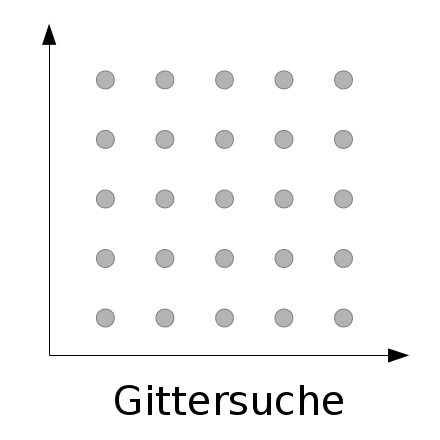
\includegraphics[scale=1.0]{images/svm/Gittersuche.png} 
	\caption{Der bei der Gittersuche verwendete Suchraster.}
	\label{fig:Gittersuche}
\end{figure}

Die Gittersuche deckt den Suchraum je nach Auflösung sehr gut ab. Sie skaliert jedoch mit \textit{O(n^k)}, wobei \textit{n} Anzahl der Stichproben pro Achse und \textit{k} der Anzahl der zu prüfenden Parameter entspricht. Für höhere Dimensionen führt dies zu einer Explosion der zu evaluierenden Parametersätze, für bis zu zwei Dimensionen liegt die Laufzeit jedoch im Rahmen des praktisch sinnvollen.

\subsubsection{DoE-Suche}
\label{subsubsec:DoE-Suche}
Bei diesem Ansatz zieht man - wie schon bei der Gittersuche - Stichproben aus dem Parameterraum und bestimmt mittels Evaluation den besten Parametersatz. Das spezielle Muster, nach dem hier die Ziehung der Stichproben erfolgt, ist der  statistische Versuchsplanung.

Diese im Englischen als \textit{Design of Experiments (DoE)} bezeichnete Wissenschaft ermöglicht es – grob erklärt – im Rahmen eines kontrollierten Experiments mehrere Stellgrößen auf einmal zu verändern und dennoch eindeutige Schlussfolgerungen aus den Ergebnissen abzuleiten. Der Zweck liegt darin, so die Anzahl der benötigten Versuche zu reduzieren.

\begin{figure}[!h]
	\centering
	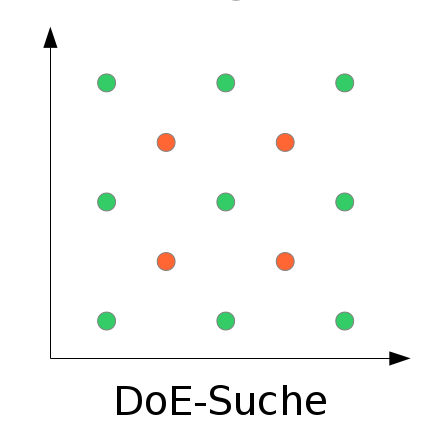
\includegraphics[scale=1.0]{images/svm/DoE-Suche.png} 
	\caption{Der bei der DoE-Suche verwendete Suchraster.}
	\label{fig:DoE-Suche}
\end{figure}

Die erzielten Ergebnisse sind qualitativ ungefähr gleichwertig zu der der Gittersuche, jedoch ist der hier beschriebene Ansatz um eine Größenordnung schneller.

\subsubsection{Multiple Iterationen}
\label{subsubsec:MultipleIterationen}
Die Genauigkeit des Parameterschätzung kann erhöht werden, indem die Parametersuche iterativ durchgeführt wird \cite{HsuLibsvmTutorial2003}. Hierzu wird das Suchfenster, also der zu untersuchende Bereich im Parameterraum (z.B. auf ein Viertel der ursprünglichen Größe) verkleinert und um den besten Punkt der letzten Iteration herum neu positioniert.

Es hat sich gezeigt, dass das Suchfenster mit der Zeit abdriften kann. Dies geschieht, wenn Teile des neuen Fensters außerhalb des alten Suchfensters liegen. Ist dies der Fall, so muss eine Positionsanpassung durchgeführt und das Fenster geringfügig verschoben werden.

Die Suche kann abgebrochen werden, wenn eine maximale Anzahl an Iterationen durchgeführt wurde oder die Änderung im MSE zur letzten Iteration unter einen vorgegebenen Schwellwert sinkt.

\subsubsection{Abdeckung des Suchraums}
\label{subsubsec:AbdeckungDesSuchraums}
Um den Parameterraum möglichst weitläufig abzudecken empfiehlt es sich, die ermittelten Parameter vor dem Training der SVM mit einer entsprechenden Funktion zu transformieren. Entsprechende Vorschläge werden in \cite{HsuLibsvmTutorial2003, Staelin2002} gemacht.

\begin{figure}[!h]
	\centering
	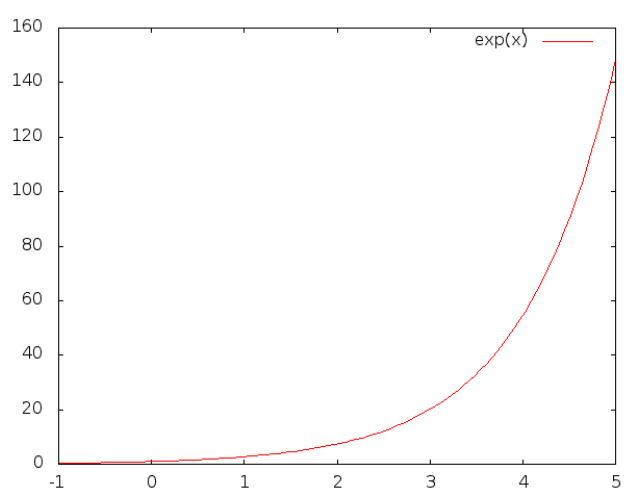
\includegraphics[scale=1.0]{images/svm/Abdeckung Suchraum.png} 
	\caption{Die durch Transformation verbesserte Abdeckung des Suchraums.}
	\label{fig:AbdeckungSuchraum}
\end{figure}

Als besonders rentabel hat sich eine Transformation mit der e-Funktion erwiesen. Hierdurch werden sowohl möglichst kleine als auch möglichst große Werte abgedeckt. In der Praxis hat sich ein Suchintervall von -5 bis 15 als rentabel erwiesen, was nach der Transformation einen Wertebereich von $10^{-3}$ bis $10^{6}$ ergibt.

\subsection{Bestimmung des Eingaberaums}
\label{subsec:BestimmungDesEingaberaums}
Von den ca. 30 zur Verfügung stehenden Merkmalen sind zwei Drittel als Eingangsgrößen geeignet.  Mittels 2D- und 3D-Plots wurden (nicht-triviale) Korrelationen zwischen den einzelnen Ein- und Ausgangsgrößen gesucht. Es konnten jedoch in den besagten Unterräumen keine klar ersichtlichen Zusammenhänge festgestellt werden. Eine Hauptkomponentenanalyse sowie die Implementierung zusätzlicher Merkmale waren angedacht, jedoch musste aus Zeitgründen darauf verzichtet werden.

Die Auswahl der für den Eingangsraum bestimmten Merkmale erfolgte manuell. Ursprünglich war die Nutzung eines Greedy-Algorithmus vorgesehen; dies erwies sich jedoch schnell als überflüssig, da plausible Merkmale aus dem Kontext der jeweiligen Ausgangsgröße zu schließen waren.

Es wurde auch Wert darauf gelegt, dass keine triviale Korrelation zwischen einer Eingangsgröße und der jeweiligen Ausgangsgröße bestehen. Ein Beispiel hierfür ist der zukünftige Lenkwinkel, der – bedenkt man die kurze Zeitspanne von 1/15 Sekunden zwischen zwei Updates – immer linear vom aktuellen Lenkwinkel abhängig ist. Selbiges gilt auch für Gas- und Bremspedal.

Die Eignung der Merkmale wurde durch eine Offline-Evaluation sichergestellt. Durch gezieltes Weglassen einzelner Merkmale ließ sich bestimmen, dass jedes der gewählten Merkmale einen großen Informationsgehalt besitzt.

Für die Ausgangsgröße \textbf{Lenkwinkel} erwiesen sich \textit{laterale Beschleunigung, Geschwindigkeit und der Winkel zum nächsten Punkt} als die am meisten relevanten Merkmale. Die Ausgangsgröße \textbf{Beschleunigung} (d.h. Gas minus Bremse) ist mit \textit{longitudinaler Beschleunigung, Geschwindigkeit und dem Abstand zum nächsten Punkt} ähnlich aufgestellt.

\subsection{Praktische Umsetzung}
\label{subsec:PraktischeUmsetzung}
Als Implementierung für die Support-Vektor-Regression wurde die Bibliothek \textit{libSVM} herangezogen. Diese ist in der Programmiersprache C verfasst und passt damit zu der im Rahmen des Projektes verwendeten Sprache C++. Die Bibliothek enthält alle benötigten Funktionen. Außerdem stellt sie neben dem Quellcode bereits lauffähige Programme zur Verfügung. Diese konnten im Rahmen von Bash-Skripten erfolgreich für Training und Evaluation eingesetzt werden.

Für die Parametersuche wurde ein separates Programm geschrieben, das die beiden weiter oben beschriebenen Verfahren zur Parameterschätzung, sowie multiple Iterationen und die Tranformation mittels der e-Funktion implementiert. Weiterhin unterstützende Bash-Skripte angefertigt, die das Training der beiden SVMs sowie deren Offline-Evaluation vollautomatisch durchführen.

Weiterhin wurde das Framework um ein entsprechendes Modul erweitert, mit dessen Unterstützung sich das Verfahren online am Fahrsimulator testen lässt. Die Implementierung ist relativ trivial gehalten, es handelt sich hierbei nur um das Setup der beiden SVMs, die Eingabe der aktuellen Merkmale, sowie die Verarbeitung und Weitergabe der Ausgabedaten an den Fahrsimulator.

\subsection{Performance}
\label{subsec:Performance}
Bei der Offline-Evaluation erzielte das Verfahren auf ungesehenen Daten einen sehr guten MSE im Bereich von $10^{-3}$. Weniger erfolgreich waren die Ergebnisse der Online-Evaluation. Das Fahrzeug folgte wenige Sekunden sowohl räumlich als auch zeitlich der vorgegebenen Trajektorie, neigte dann jedoch zu einer stetigen Kreisfahrt, da die beiden SVMs für Beschleunigung und Stellgröße ihre Ausgaben nicht oder nur noch minimal änderten.

Als Grund hierfür konnten unzureichende Trainingsdaten ermittelt werden. Die SVMs wurden mit Eingabewerten konfrontiert, die in dieser Form nicht in den Testdaten vorhanden waren. Folglich ist in diesem Bereich auch nicht mit einer Generalisierung zu rechnen. Es handelt sich hierbei um vom Lernverfahren unabhängiges Problem, dass durch zusätzliche Lerndaten hätte gelöst werden können.

% section Verfahren5 (end)


% chapter Verfahren (end)